\section{Team}

The datasets were downloaded and executed using the following commands:

\begin{minted}{console}
./run_docker.sh orbslam:latest
./run_docker.sh kimera:latest
\end{minted}

Fig.~\ref{fig:runtime} shows the runtime output of both systems.

\subsection*{Deliverable 6 - Performance Comparison}

Before comparing trajectories, we ran \lstinline{fix_timestamps.py} to correct the timestamp files. We then used the \lstinline{evo_traj} tool to generate the initial comparison plot:

\begin{minted}{console}
evo_traj tum output/kimera/kimera.txt output/orbslam/orb_slam3.txt --plot
\end{minted}

The results are shown in Fig.~\ref{fig:without_align}. Without alignment, the trajectories from blue Kimera and green ORB-SLAM3 exist in separate spatial coordinates. This is expected, as each algorithm initializes its own world frame upon startup. The 3D Trajectory and XYZ plots clearly show different starting points and orientations. The RPY plot indicates a large, constant offset in yaw (around $150^{\circ}$), while roll and pitch estimates are closer, likely due to gravity alignment. Interestingly, the Speed plot shows that both algorithms produce very similar velocity estimates, suggesting they are both tracking the drone's motion dynamics accurately, despite the coordinate mismatch.

Next, we aligned the trajectories to the ground truth data. First, the ground truth file was converted to TUM format:

\begin{minted}{console}
evo_traj euroc ~/datasets/vnav/MH_01_easy/mav0/state_groundtruth_estimate0/data.csv --save_as_tum
\end{minted}

Then, the comparison was run with alignment enabled:

\begin{minted}{console}
evo_traj tum output/kimera/kimera.txt output/orbslam/orb_slam3.txt --ref data.tum --plot --align
\end{minted}

The aligned results are in Fig.~\ref{fig:with_align}. After alignment, both estimated trajectories closely follow the ground truth reference. The 3D and XYZ plots show minimal drift, even during the MAV's complex maneuvers. The RPY plots confirm that both algorithms accurately capture rapid changes in attitude. The Speed plot reveals that while both estimates contain some high-frequency noise—common in IMU-based predictions—they reliably track the overall velocity profile of the ground truth. These results demonstrate that both ORB-SLAM3 and Kimera provide reliable state estimation on the EuRoC dataset.

\subsection*{[Optional] Deliverable 7 - LDSO}

We also ran LDSO (LiDAR-Direct-Sparse-Odometry) on the EuRoC dataset. Fig.~\ref{fig:ldso_run} shows a snapshot from the viewer, displaying the reconstructed sparse 3D point cloud, active keyframes, and the current camera pose. The semi-dense map effectively captures the structural details of the Machine Hall environment.

\begin{figure*}[!t]
  \centering
  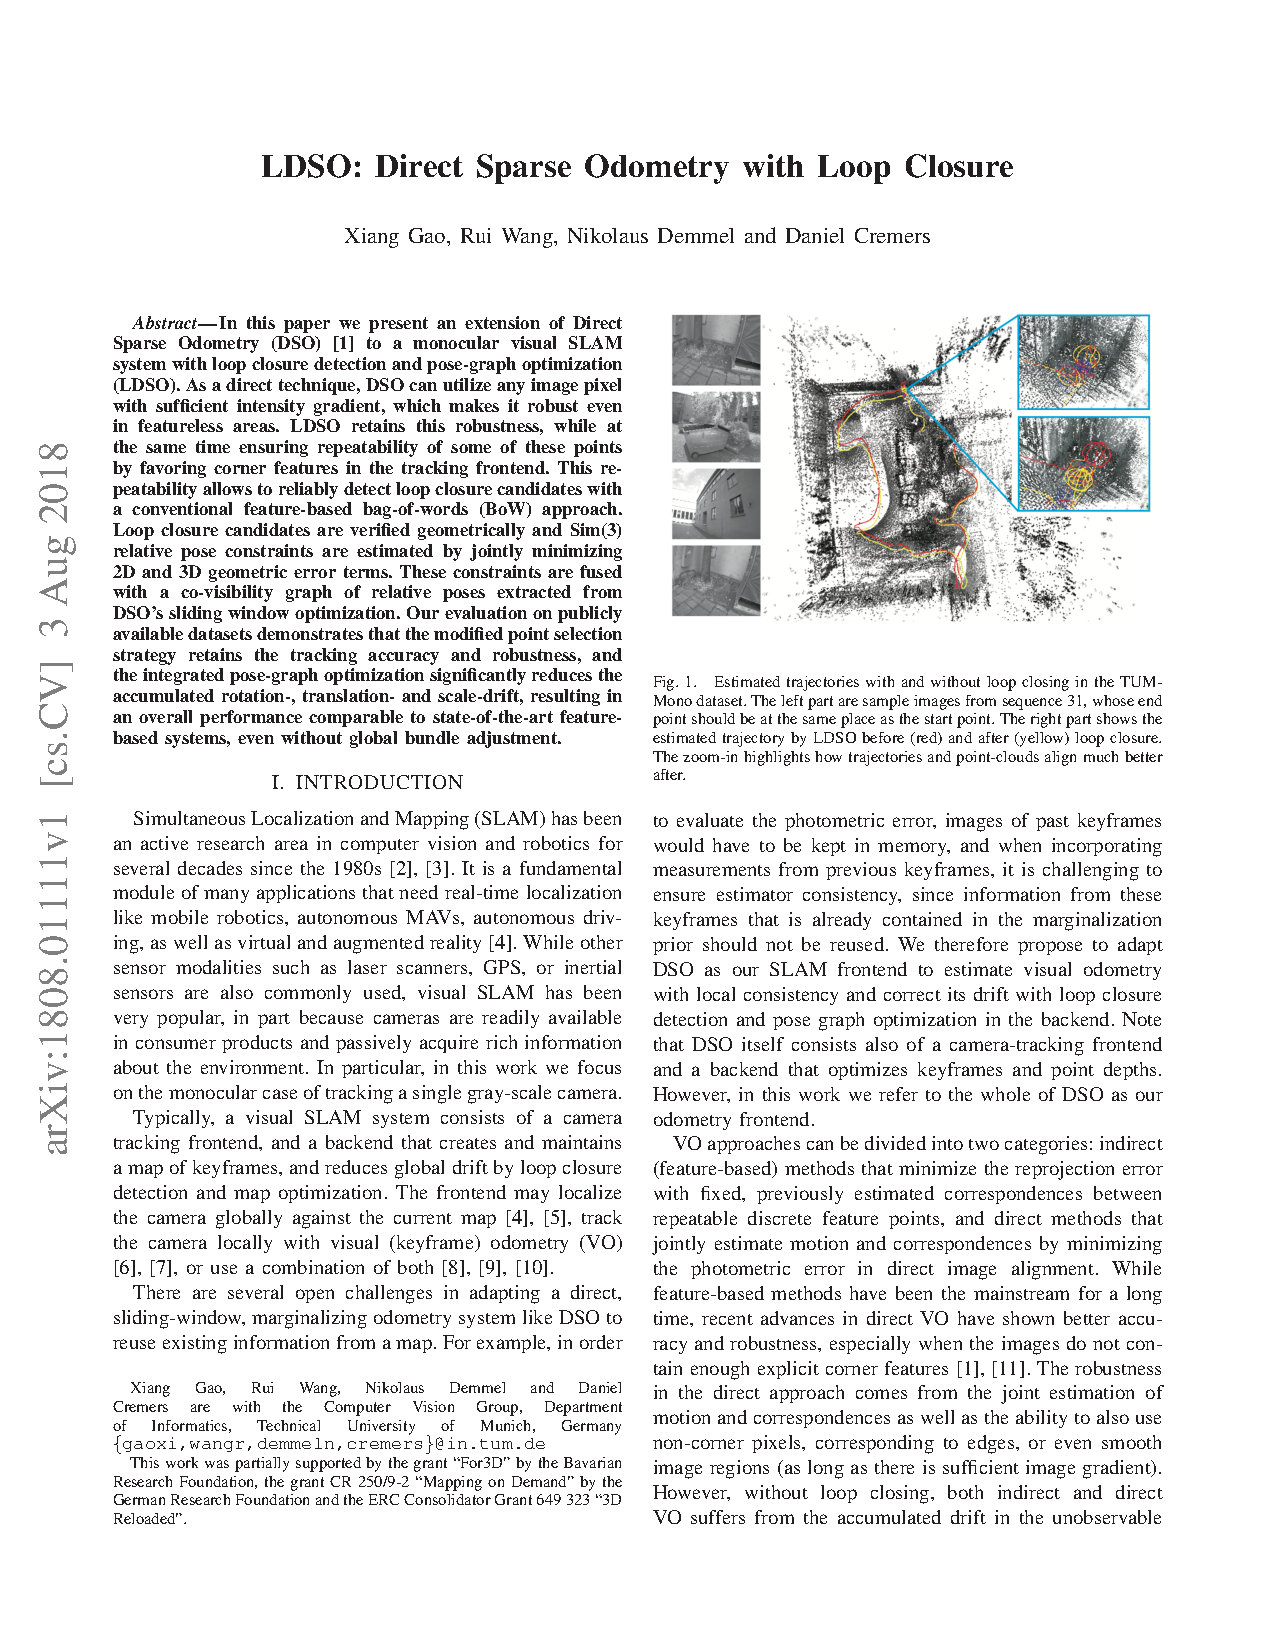
\includegraphics[width=0.8\linewidth]{figures/LDSO}
  \caption{Runtime snapshot of the LDSO pipeline.}
  \label{fig:ldso_run}
  \hrulefill
  \vspace*{4pt}
\end{figure*}

LDSO is a monocular, direct visual odometry method. A known limitation of monocular systems is scale ambiguity—they cannot recover the absolute metric scale of the world. Therefore, to fairly compare its trajectory against the ground truth and the stereo/VIO systems (Kimera and ORB-SLAM3), we must perform a Sim(3) alignment. This corrects for differences in rotation, translation, and scale. We used the \lstinline{--correct_scale} flag in \lstinline{evo} for this purpose.

Fig.~\ref{fig:ldso_comp} presents the comparison results. Several key points stand out:

\paragraph{Trajectories} After scale correction, the LDSO trajectory (blue, labeled `results\_final`) aligns very well with the ground truth, Kimera, and ORB-SLAM3. This shows that even without IMU or stereo data, LDSO's direct photometric optimization can accurately reconstruct the camera's path in a feature-rich environment like EuRoC.

\paragraph{XYZ} The LDSO position estimates appear smooth. Direct methods utilize intensity gradients from most pixels, which can lead to robust tracking, though they are also more sensitive to lighting changes and photometric calibration.

\paragraph{RPY} LDSO's roll, pitch, and yaw estimates track the ground truth well. Unlike VIO systems which have direct accelerometer measurements to constrain roll and pitch, monocular VO can drift in these axes over time. For this sequence, however, LDSO maintains stable orientation estimates.

\paragraph{Speeds} The velocity profile derived from the scaled LDSO trajectory matches those from the VIO pipelines. This indicates good temporal consistency in its pose estimates—the scaled monocular velocities correspond well to real-world motion.

\subsection*{Summary of Team Deliverables}

\paragraph{Comparison plots of Kimera and ORB-SLAM3 on \lstinline{MH_01_easy} with comments on differences in trajectories} The ``Spy Game'' assignment mathematically demonstrated that the full SLAM problem could theoretically be reduced to a rotation-only optimization problem, decreasing the number of variables from \(6N+3M\) to \(3N\). However, this simplification comes with a significant computational drawback: the loss of sparsity in the system. Visually, marginalizing landmarks creates dense blocks (fill-in) in the information matrix. While solving a large sparse system typically scales as \(O(N)\), solving the reduced but dense system becomes \(O(N^3)\). This explains why modern backends (like the \(g^2o\) library used in ORB-SLAM and LSD-SLAM) do not naively eliminate all landmarks. Instead, they preserve and exploit the inherent sparse block structure of the Bundle Adjustment problem to maintain real-time efficiency.

\paragraph{Plot of Kimera and ORB-SLAM3 trajectories on \lstinline{MH_01_easy} aligned with ground-truth with comments on any differences in the trajectories} Comparing ORB-SLAM/Kimera (feature-based) with LDSO (direct) illustrates a fundamental design trade-off. Feature-based methods rely on detecting and matching distinctive keypoints (e.g., ORB descriptors), which provides robustness against illumination changes and viewpoint variations. In contrast, direct methods like LDSO optimize for photometric consistency across pixels, which can yield smoother trajectories and denser reconstructions but assumes consistent brightness and is more vulnerable to auto-exposure or lighting variations. While LDSO produced a semi-dense map useful for environmental understanding, ORB-SLAM's sparse map is more computationally efficient for long-term tracking.

\paragraph{[Optional] Plot of Kimera + ORB-SLAM3 + LDSO (aligned and scale corrected with ground-truth) with comments on any differences in trajectories} The experiments clearly highlight the limitation of monocular visual odometry: scale ambiguity. While the trajectory shape estimated by monocular LDSO was correct, its absolute scale was arbitrary, requiring Sim(3) alignment (scale correction) for meaningful comparison with ground truth and metric systems like stereo ORB-SLAM and VIO Kimera. This underscores the critical advantage of sensor fusion (visual-inertial) or stereo vision in robotics applications. For monocular systems, scale drift remains inevitable over long trajectories unless corrected through loop closures with Sim(3) optimization, as implemented in systems like LSD-SLAM.
